\chapter{Configuration}
The user interface is designed to be flexible and configurable in the most possible aspects. Configuration Files are written in JSON[json.org] and can be used to adapt the interface to the own specific needs. The general configuration structure is shown in figure \ref{fig:configstruct}. How to work with the interface and create configuration files will be explained in the following.

\section{Default-Configuration File}
The Default-Configuration file located in "config/gui{\_}default.cfg" holds default values for each type of object and almost every possible property. It gives a good example on how a configuration should look like, because it is important to keep the hierarchical structure. When creating own configurations, left out values will be automatically replaced with the values set in the default file, thus allowing to craft own configurations easily and with little effort. Note that any changes on the default file can prevent the interface from running, for example removing values that are needed as default references.

\begin{figure} [h]
\centering
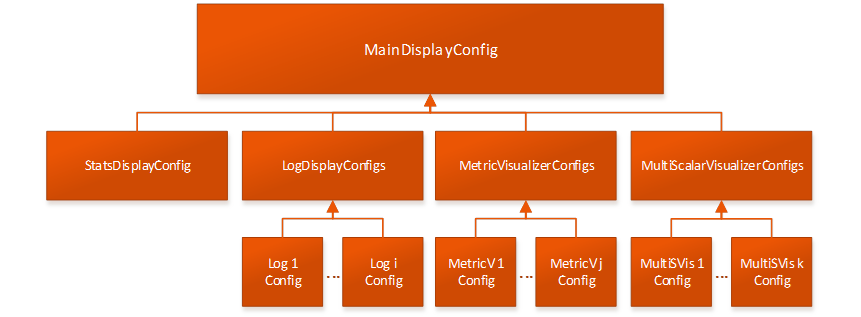
\includegraphics [scale=1] {images/configstruct}
\caption{Configuration Structure.}
\label{fig:configstruct}
\end{figure}

\section{Building own configuration files}
When creating an own configuration file it is recommended to take a look at the minimal display configuration located in "config/gui{\_}min.cfg" and to expand it for your own needs. It uses only the minimum of values needed to create a useful interface, see figure \ref{fig:mincfg}. It creates a MainDisplay (1) in Playback-Mode (1.1) checking the relative directory "data/test123/run.0/" (1.2). It consists of a StatsDisplay (2), a MetricVisualizer (3) and a MultiScalarVisualizer (4). For the latter two, only the names and positions are defined. See figure \ref{fig:mincfgex} on the next page for the resulting Interface. For more sophisticated settings check the "config/displayConfig.cfg".

\begin{figure} [h]
\centering
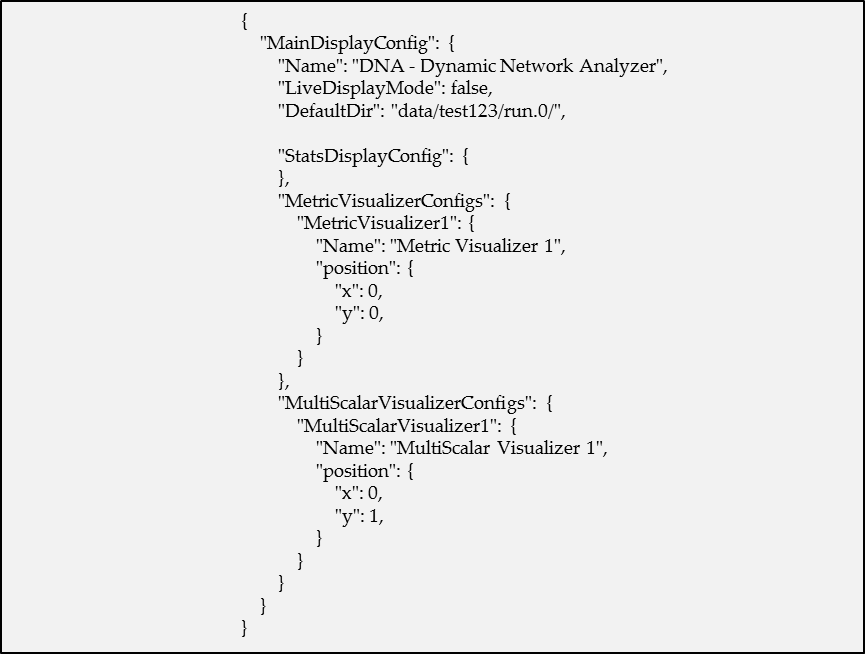
\includegraphics [scale=1] {images/mincfg}
\caption{Minimal-Configuration-File ("config/gui{\_}min.cfg").}
\label{fig:mincfg}
\end{figure}

\begin{figure} [h]
\centering
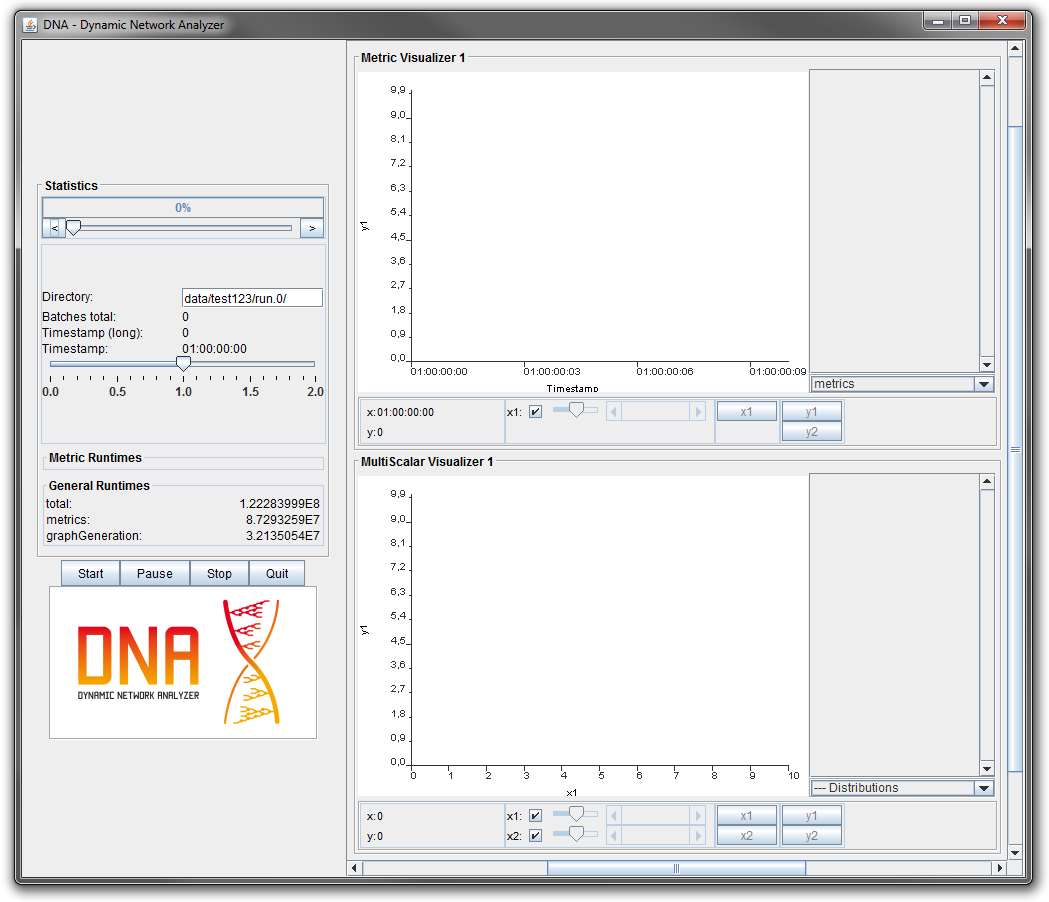
\includegraphics [scale=0.5] {images/mincfgex}
\caption{Resulting Interface from the Minimal-Configuration-File ("config/gui{\_}min.cfg").}
\label{fig:mincfgex}
\end{figure}

\subsection{Adjusting the MetricVisualizer}
In the following example we will extend the minimal configuration from the previous chapter by adjusting the MetricVisualizer. The "displayConfig.cfg" configuration file helps us to see what values can be adjusted to fulfill our needs. First we might always want the amount of nodes and edges to be displayed in the chart on the second y-axis. This is done by adding a VisualizerConfig (1) object, which itself holds two SingleConfigs (2) \& (3), one for each value. See figure \ref{fig:metricvis2}, the added code is highlighted in red.

\begin{figure} [h]
\centering
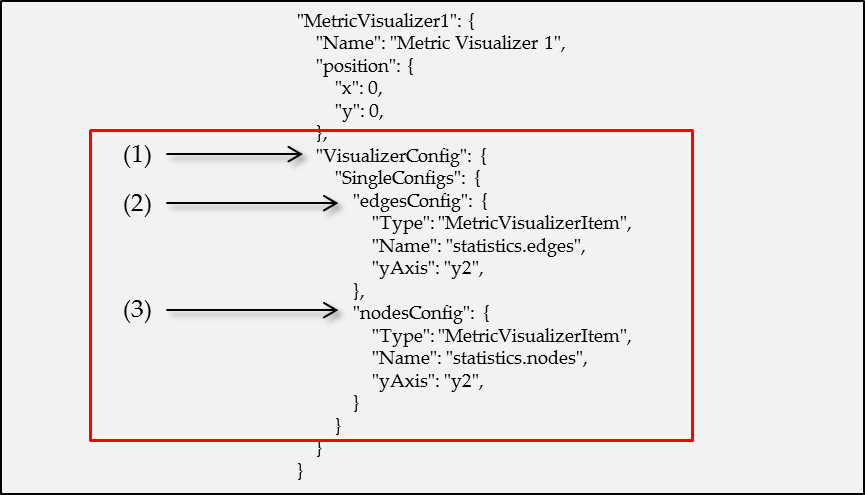
\includegraphics [scale=1] {images/metricvis2}
\caption{Extended MetricVisualizer example.}
\label{fig:metricvis2}
\end{figure}

Now we might want to add a specific type of value to be added to the chart by default on startup. This is done by adding „GeneralConfigs“ to the previous defined VisualizerConfig object. They are applied for each value of a specific kind. Possible general configs are "generalMetricConfig", "generalGeneralRuntimesConfig", "generalStatisticsConfig", "generalMetricRuntimesConfig"“, "generalDistributionConfig", and "generalNodeValueListConfig". For example to add all available metrics by default, we add a "generalMetricConfig" (1). Figure \ref{fig:metricvis3} shows which code has been added to plot all metrics as linespoint (2) on the left y-Axis in hidden-mode (3). This allows the user to have all metrics available in the chart and to simply show those he wants with a single mouse-click on the red "H". Figure \ref{fig:metricvis4} on the next page shows the resulting MetricVisualizer.

\begin{figure} [h]
\centering
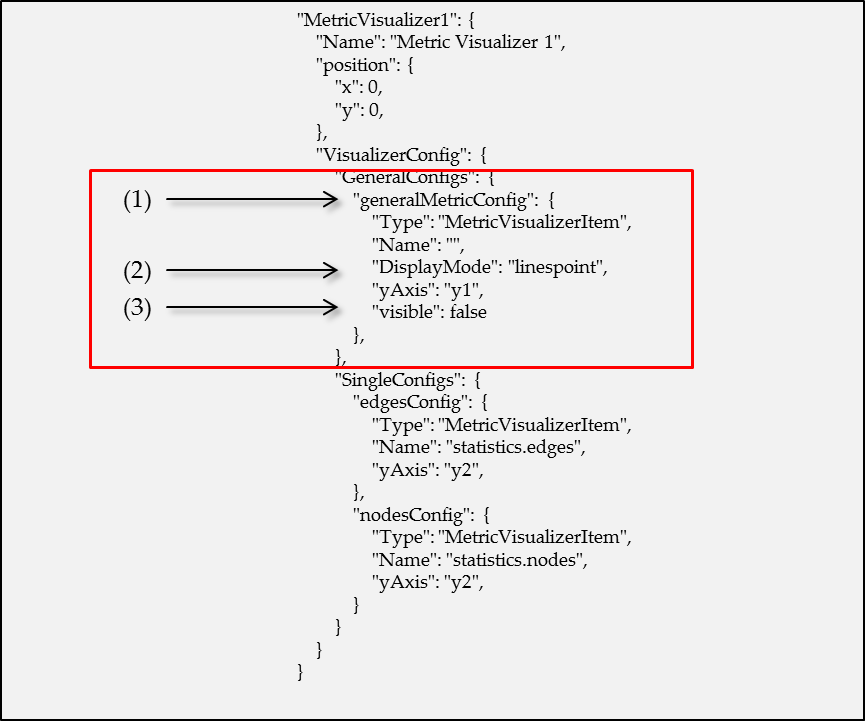
\includegraphics [scale=1] {images/metricvis3}
\caption{Further extended MetricVisualizer example.}
\label{fig:metricvis3}
\end{figure}

\begin{figure} [h]
\centering
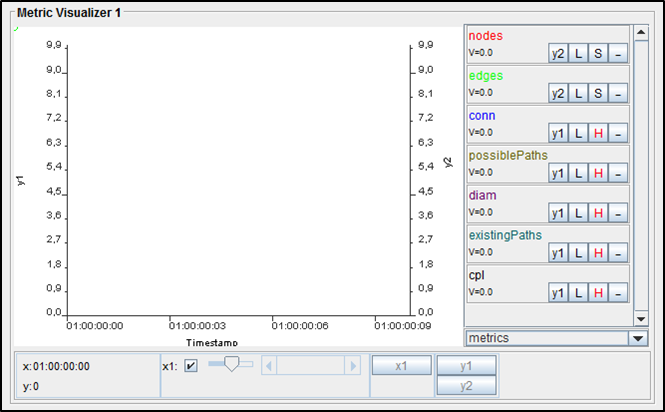
\includegraphics [scale=1] {images/metricvis4}
\caption{Resulting Interface from the further extended MetricVisualizer example.}
\label{fig:metricvis4}
\end{figure}

\textbf{Note:} All values that are added to the legend are existent in the chart, even if they are in hidden mode. Therefore the axis scaling and offsets might interfere with the expected outcome of your configuration. The MultiScalar Visualizer can be adjusted analogously to the MetricVisualizer.

\subsection{Positioning in Data-Display Area}
The data display area can be pictured as a grid, see figure \ref{fig:metricvis5}. By default each object will be assigned to one square of the grid, regarding it‘s
(x,y)-coordinates. Additionally it is possible to set row-/colspan values for each object, allowing them to fill more than one row or column. Table \ref{tab:grid1} shows which configuration is needed to build the area from figure \ref{fig:metricvis5}. Note that the grid-sizes are relative and will be dynamically adapted to the largest object in the respective row / column.

\begin{figure} [h]
\centering
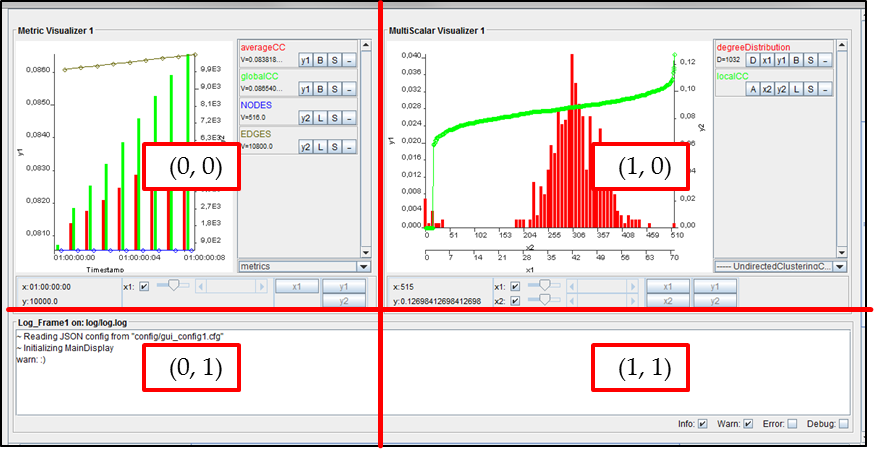
\includegraphics [scale=1] {images/metricvis5}
\caption{The data display grid.}
\label{fig:metricvis5}
\end{figure}

\begin{table}[h]
\centering
\begin{tabular}[h]{|l|l|l|l|l|}\hline
	\textbf{Object} & \textbf{X} & \textbf{Y} & \textbf{Rowspan} & \textbf{Colspan}\\
	\hline
	MetricVisualizer 1 & 0 & 0 & 1 & 1\\
	\hline
	MultiScalar Visualizer 1 & 1 & 0 & 1 & 1\\
	\hline
	Log\textunderscore Frame1 & 0 & 1 & 1 & 2\\
	\hline
\end{tabular}
\caption{Objects and their properties from the example in figure \ref{fig:metricvis5}}
\label{tab:grid1}
\end{table}